% Options for packages loaded elsewhere
\PassOptionsToPackage{unicode}{hyperref}
\PassOptionsToPackage{hyphens}{url}
%
\documentclass[
]{article}
\usepackage{lmodern}
\usepackage{amssymb,amsmath}
\usepackage{ifxetex,ifluatex}
\ifnum 0\ifxetex 1\fi\ifluatex 1\fi=0 % if pdftex
  \usepackage[T1]{fontenc}
  \usepackage[utf8]{inputenc}
  \usepackage{textcomp} % provide euro and other symbols
\else % if luatex or xetex
  \usepackage{unicode-math}
  \defaultfontfeatures{Scale=MatchLowercase}
  \defaultfontfeatures[\rmfamily]{Ligatures=TeX,Scale=1}
\fi
% Use upquote if available, for straight quotes in verbatim environments
\IfFileExists{upquote.sty}{\usepackage{upquote}}{}
\IfFileExists{microtype.sty}{% use microtype if available
  \usepackage[]{microtype}
  \UseMicrotypeSet[protrusion]{basicmath} % disable protrusion for tt fonts
}{}
\makeatletter
\@ifundefined{KOMAClassName}{% if non-KOMA class
  \IfFileExists{parskip.sty}{%
    \usepackage{parskip}
  }{% else
    \setlength{\parindent}{0pt}
    \setlength{\parskip}{6pt plus 2pt minus 1pt}}
}{% if KOMA class
  \KOMAoptions{parskip=half}}
\makeatother
\usepackage{xcolor}
\IfFileExists{xurl.sty}{\usepackage{xurl}}{} % add URL line breaks if available
\IfFileExists{bookmark.sty}{\usepackage{bookmark}}{\usepackage{hyperref}}
\hypersetup{
  pdftitle={Tarea 2: Modelos lineales generalizados y paramétricos},
  pdfauthor={Angie Rodriguez Duque \& Cesar Saavedra Vanegas},
  hidelinks,
  pdfcreator={LaTeX via pandoc}}
\urlstyle{same} % disable monospaced font for URLs
\usepackage[margin=1in]{geometry}
\usepackage{color}
\usepackage{fancyvrb}
\newcommand{\VerbBar}{|}
\newcommand{\VERB}{\Verb[commandchars=\\\{\}]}
\DefineVerbatimEnvironment{Highlighting}{Verbatim}{commandchars=\\\{\}}
% Add ',fontsize=\small' for more characters per line
\usepackage{framed}
\definecolor{shadecolor}{RGB}{248,248,248}
\newenvironment{Shaded}{\begin{snugshade}}{\end{snugshade}}
\newcommand{\AlertTok}[1]{\textcolor[rgb]{0.94,0.16,0.16}{#1}}
\newcommand{\AnnotationTok}[1]{\textcolor[rgb]{0.56,0.35,0.01}{\textbf{\textit{#1}}}}
\newcommand{\AttributeTok}[1]{\textcolor[rgb]{0.77,0.63,0.00}{#1}}
\newcommand{\BaseNTok}[1]{\textcolor[rgb]{0.00,0.00,0.81}{#1}}
\newcommand{\BuiltInTok}[1]{#1}
\newcommand{\CharTok}[1]{\textcolor[rgb]{0.31,0.60,0.02}{#1}}
\newcommand{\CommentTok}[1]{\textcolor[rgb]{0.56,0.35,0.01}{\textit{#1}}}
\newcommand{\CommentVarTok}[1]{\textcolor[rgb]{0.56,0.35,0.01}{\textbf{\textit{#1}}}}
\newcommand{\ConstantTok}[1]{\textcolor[rgb]{0.00,0.00,0.00}{#1}}
\newcommand{\ControlFlowTok}[1]{\textcolor[rgb]{0.13,0.29,0.53}{\textbf{#1}}}
\newcommand{\DataTypeTok}[1]{\textcolor[rgb]{0.13,0.29,0.53}{#1}}
\newcommand{\DecValTok}[1]{\textcolor[rgb]{0.00,0.00,0.81}{#1}}
\newcommand{\DocumentationTok}[1]{\textcolor[rgb]{0.56,0.35,0.01}{\textbf{\textit{#1}}}}
\newcommand{\ErrorTok}[1]{\textcolor[rgb]{0.64,0.00,0.00}{\textbf{#1}}}
\newcommand{\ExtensionTok}[1]{#1}
\newcommand{\FloatTok}[1]{\textcolor[rgb]{0.00,0.00,0.81}{#1}}
\newcommand{\FunctionTok}[1]{\textcolor[rgb]{0.00,0.00,0.00}{#1}}
\newcommand{\ImportTok}[1]{#1}
\newcommand{\InformationTok}[1]{\textcolor[rgb]{0.56,0.35,0.01}{\textbf{\textit{#1}}}}
\newcommand{\KeywordTok}[1]{\textcolor[rgb]{0.13,0.29,0.53}{\textbf{#1}}}
\newcommand{\NormalTok}[1]{#1}
\newcommand{\OperatorTok}[1]{\textcolor[rgb]{0.81,0.36,0.00}{\textbf{#1}}}
\newcommand{\OtherTok}[1]{\textcolor[rgb]{0.56,0.35,0.01}{#1}}
\newcommand{\PreprocessorTok}[1]{\textcolor[rgb]{0.56,0.35,0.01}{\textit{#1}}}
\newcommand{\RegionMarkerTok}[1]{#1}
\newcommand{\SpecialCharTok}[1]{\textcolor[rgb]{0.00,0.00,0.00}{#1}}
\newcommand{\SpecialStringTok}[1]{\textcolor[rgb]{0.31,0.60,0.02}{#1}}
\newcommand{\StringTok}[1]{\textcolor[rgb]{0.31,0.60,0.02}{#1}}
\newcommand{\VariableTok}[1]{\textcolor[rgb]{0.00,0.00,0.00}{#1}}
\newcommand{\VerbatimStringTok}[1]{\textcolor[rgb]{0.31,0.60,0.02}{#1}}
\newcommand{\WarningTok}[1]{\textcolor[rgb]{0.56,0.35,0.01}{\textbf{\textit{#1}}}}
\usepackage{longtable,booktabs}
% Correct order of tables after \paragraph or \subparagraph
\usepackage{etoolbox}
\makeatletter
\patchcmd\longtable{\par}{\if@noskipsec\mbox{}\fi\par}{}{}
\makeatother
% Allow footnotes in longtable head/foot
\IfFileExists{footnotehyper.sty}{\usepackage{footnotehyper}}{\usepackage{footnote}}
\makesavenoteenv{longtable}
\usepackage{graphicx,grffile}
\makeatletter
\def\maxwidth{\ifdim\Gin@nat@width>\linewidth\linewidth\else\Gin@nat@width\fi}
\def\maxheight{\ifdim\Gin@nat@height>\textheight\textheight\else\Gin@nat@height\fi}
\makeatother
% Scale images if necessary, so that they will not overflow the page
% margins by default, and it is still possible to overwrite the defaults
% using explicit options in \includegraphics[width, height, ...]{}
\setkeys{Gin}{width=\maxwidth,height=\maxheight,keepaspectratio}
% Set default figure placement to htbp
\makeatletter
\def\fps@figure{htbp}
\makeatother
\setlength{\emergencystretch}{3em} % prevent overfull lines
\providecommand{\tightlist}{%
  \setlength{\itemsep}{0pt}\setlength{\parskip}{0pt}}
\setcounter{secnumdepth}{-\maxdimen} % remove section numbering

\title{Tarea 2: Modelos lineales generalizados y paramétricos}
\author{Angie Rodriguez Duque \& Cesar Saavedra Vanegas}
\date{Octubre 22 de 2020}

\begin{document}
\maketitle

\hypertarget{actividad-1}{%
\section{Actividad 1}\label{actividad-1}}

\hypertarget{section}{%
\subsection{}\label{section}}

Se dispone de los tiempos de vida (tiempos hasta que fallan, en horas)
de \(49\) recipientes de presión sometidos a un nivel de carga del
\(70\%\)

\hypertarget{distribuciuxf3n-weibull}{%
\subsection{Distribución Weibull}\label{distribuciuxf3n-weibull}}

Para estudiar este tipo de variable se acostumbra utilizar la
distribución de Weibull, cuya función de densidad es:

\[f(y;\lambda,\theta)=\displaystyle\frac{\lambda y^{\lambda-1}}{\theta^{\lambda}}exp \left[-\left(\frac{y}{\theta}\right)^{\lambda}\right] \]

Para analizar este problema usaremos el método de Newton (conocido
también como el método de Newton Raphson o el método de Newton Fourier),
el cual es un algoritmo basado en la derivada que permite encontrar
aproximaciones de los ceros o raíces de una función real derivable. En
este caso particular se hara uso de la función U de scoring para la
Weibul y se asumira \(\lambda\) conocido y \(U\) será el estimador
\(\hat\theta\) del parametro de escala \(\theta\).

\begin{enumerate}
\def\labelenumi{\arabic{enumi}.}
\item
  Se elige \(x_{0}\) en el eje de las \(x\), asumiendo que está cerca de
  la solución de \(f(x)=0\) (raíz buscada)
\item
  Calculamos la ecuación punto pendiente de la recta tangente a la
  función en \((x_{0},f(x_{0}))\), a saber
  \(y−f(x_{0})=f′(x_{0})(x−x_{0})\) (1)
\item
  Esta recta debe intersecar al eje de las \(x\), en un punto más
  cercano a la raíz buscada; en el punto \((x_{1},0)\).
\item
  El punto \((x_{1},0)\) satisface la ecuación (1) y sustituyendo, queda
  (2): \[0−f(x0)=f′(x0)(x−x0)\]
\item
  Si \(f(x0)=0\), entonces despejando \(x_{1}\) en (2) se obtiene:
\end{enumerate}

\[x_{1}=x_{0}−\frac{f(x_{0})}{f′(x_{0})}\]

\begin{enumerate}
\def\labelenumi{\arabic{enumi}.}
\setcounter{enumi}{5}
\item
  Repetimos el procedimiento anterior para \(x_{0}\), pero ahora
  comenzando con \(x_{1}\), en cuyo caso se obtiene
  \(x_{2}=x_{1}−\frac{f(x_{1})}{f′(x_{1})}\). De forma que \(x_{2}\)
  está más cerca de la raíz buscada que \(x\).
\item
  Iterando cada vez con el número obtenido, se construye una secuencia:
  \(x_{0},x_{1},x−2,…,x_{n},…\) de números cada vez más próximos a la
  raíz, tales que: \[x_{n+1}=x_{n}−\frac{f(x_{n})}{f′(x_{n})}\]
\end{enumerate}

Siguiendo este algoritmo y realizando su representación en R se obtienen
los siguientes resultados para \(\lambda=2\):\#\# Función U de scoring
para la Weibull

\[ \frac{dl}{d\theta}=U=\displaystyle\sum_{i=1}^{N}\left[ \frac{-\lambda}{\theta}+\frac{\lambda y^{\lambda}_{i}}{\theta^{\lambda+1}}\right]\]
Como asumimos que conocemos \(\lambda\), la solución de \(U=0\) será el
estimador \(\hat{\theta}\) del parámetro de escala \(\theta\).

\hypertarget{funciuxf3n-u-de-scoring-para-la-weibull-con-lambda2}{%
\subsubsection{\texorpdfstring{Función U de scoring para la Weibull con
\(\lambda=2\)}{Función U de scoring para la Weibull con \textbackslash lambda=2}}\label{funciuxf3n-u-de-scoring-para-la-weibull-con-lambda2}}

Como en este caso estamos asumiendo que \(\lambda=2\), entonces la
expresión anterior será aplicable en este caso.

\[U=\frac{2\cdot 36}{\theta}+\frac{2\cdot \displaystyle\sum_{i=1}^{36}y^{2}_{i}}{\theta^{3}}\]
Nos proponemos encontrar \(\theta\) tal que \(U=0\)

\hypertarget{el-muxe9todo-de-newton-raphson}{%
\subsubsection{El método de
Newton-Raphson}\label{el-muxe9todo-de-newton-raphson}}

\hypertarget{actividad-2}{%
\section{Actividad 2}\label{actividad-2}}

\hypertarget{base-de-datos}{%
\subsection{Base de datos}\label{base-de-datos}}

\begin{Shaded}
\begin{Highlighting}[]
\KeywordTok{dim}\NormalTok{(Datos)}
\end{Highlighting}
\end{Shaded}

\begin{verbatim}
## [1] 1599   12
\end{verbatim}

Este conjunto de datos de vino tinto consta de 1599 observaciones y 12
variables, 11 de las cuales son sustancias químicas. Las variables son:

\begin{enumerate}
\def\labelenumi{\arabic{enumi}.}
\item
  \textbf{Acidez fija:} La mayoría de los ácidos implicados en el vino
  son fijos o no volátiles (no se evaporan fácilmente).
\item
  \textbf{Acidez volátil:} La cantidad de ácido acético en el vino, que
  en niveles demasiado altos puede provocar un sabor desagradable a
  vinagre.
\item
  \textbf{Ácido cítrico:} Encontrado en pequeñas cantidades, el ácido
  cítrico puede agregar ``frescura'' y sabor a los vinos.
\item
  \textbf{Azúcar residual:} Es la cantidad de azúcar que queda después
  de que se detiene la fermentación, es raro encontrar vinos con menos
  de 1 gramo / litro y los vinos con más de 45 gramos / litro se
  consideran dulces.
\item
  \textbf{Cloruros:} Es la cantidad de sal del vino.
\item
  \textbf{Dióxido de azufre libre:} La forma libre de \(SO_{2}\) existe
  en equilibrio entre el \(SO_{2}\) molecular (como gas disuelto) y el
  ion bisulfito; Previene el crecimiento microbiano y la oxidación del
  vino.
\item
  \textbf{Dióxido de azufre total:} Es la cantidad de formas libres y
  unidas de \(SO_{2}\); en concentraciones bajas, el \(SO_{2}\) es
  mayormente indetectable en el vino, pero en concentraciones de
  \(SO_{2}\) libre superiores a 50 ppm, el \(SO_{2}\) se hace evidente
  en la nariz y el sabor del vino.
\item
  \textbf{Densidad:} La densidad es cercana a la del agua dependiendo
  del porcentaje de alcohol y contenido de azúcar.
\item
  \textbf{pH:} Describe qué tan ácido o básico es un vino en una escala
  de 0 (muy ácido) a 14 (muy básico); la mayoría de los vinos están
  entre 3-4 en la escala de pH.
\item
  \textbf{Sulfatos:} Aditivo del vino que puede contribuir a los niveles
  de dióxido de azufre \((SO_{2})\), que actúa como antimicrobiano y
  antioxidante.
\item
  \textbf{Alcohol:} El porcentaje de contenido de alcohol del vino.
\item
  \textbf{Calidad:} Variable de respuesta (basada en datos sensoriales,
  puntuación entre 0 y 10).
\end{enumerate}

\hypertarget{estaduxedsticas-descriptivas}{%
\subsection{Estadísticas
descriptivas}\label{estaduxedsticas-descriptivas}}

\begin{Shaded}
\begin{Highlighting}[]
\KeywordTok{summary}\NormalTok{(Datos)}
\end{Highlighting}
\end{Shaded}

\begin{verbatim}
##  fixed.acidity   volatile.acidity  citric.acid    residual.sugar  
##  Min.   : 4.60   Min.   :0.1200   Min.   :0.000   Min.   : 0.900  
##  1st Qu.: 7.10   1st Qu.:0.3900   1st Qu.:0.090   1st Qu.: 1.900  
##  Median : 7.90   Median :0.5200   Median :0.260   Median : 2.200  
##  Mean   : 8.32   Mean   :0.5278   Mean   :0.271   Mean   : 2.539  
##  3rd Qu.: 9.20   3rd Qu.:0.6400   3rd Qu.:0.420   3rd Qu.: 2.600  
##  Max.   :15.90   Max.   :1.5800   Max.   :1.000   Max.   :15.500  
##    chlorides       free.sulfur.dioxide total.sulfur.dioxide    density      
##  Min.   :0.01200   Min.   : 1.00       Min.   :  6.00       Min.   :0.9901  
##  1st Qu.:0.07000   1st Qu.: 7.00       1st Qu.: 22.00       1st Qu.:0.9956  
##  Median :0.07900   Median :14.00       Median : 38.00       Median :0.9968  
##  Mean   :0.08747   Mean   :15.87       Mean   : 46.47       Mean   :0.9967  
##  3rd Qu.:0.09000   3rd Qu.:21.00       3rd Qu.: 62.00       3rd Qu.:0.9978  
##  Max.   :0.61100   Max.   :72.00       Max.   :289.00       Max.   :1.0037  
##        pH          sulphates         alcohol         quality     
##  Min.   :2.740   Min.   :0.3300   Min.   : 8.40   Min.   :3.000  
##  1st Qu.:3.210   1st Qu.:0.5500   1st Qu.: 9.50   1st Qu.:5.000  
##  Median :3.310   Median :0.6200   Median :10.20   Median :6.000  
##  Mean   :3.311   Mean   :0.6581   Mean   :10.42   Mean   :5.636  
##  3rd Qu.:3.400   3rd Qu.:0.7300   3rd Qu.:11.10   3rd Qu.:6.000  
##  Max.   :4.010   Max.   :2.0000   Max.   :14.90   Max.   :8.000
\end{verbatim}

\begin{figure}
\centering
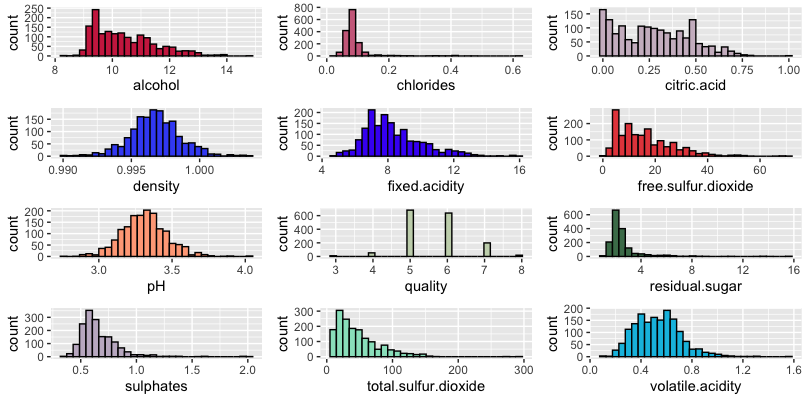
\includegraphics[width=6.77083in,height=\textheight]{G1.png}
\caption{Distribución de las variables}
\end{figure}

\hypertarget{observaciones}{%
\subsubsection{Observaciones:}\label{observaciones}}

\begin{itemize}
\item
  Algunas de las variables tienen distribuciones normales (densidad,
  acidez fija, pH, acidez volátil).
\item
  Algunas variables están un poco sesgadas hacia el extremo inferior de
  los valores (cloruros, ácido cítrico, azúcar residual, dióxido de
  azufre total).
\item
  La variable calidad tiene solo 6 valores discretos.
\end{itemize}

\begin{Shaded}
\begin{Highlighting}[]
\KeywordTok{corrplot}\NormalTok{(}\KeywordTok{cor}\NormalTok{(Datos), }\DataTypeTok{method =} \StringTok{"square"}\NormalTok{)}
\end{Highlighting}
\end{Shaded}

\begin{center}\includegraphics{Informe_files/figure-latex/unnamed-chunk-7-1} \end{center}

\begin{itemize}
\item
  La densidad tiene una correlación muy fuerte con la acidez fija.
\item
  Las variables más fuertemente correlacionadas con la calidad son la
  acidez volátil y el alcohol.
\item
  El alcohol tiene una correlación negativa con la densidad. Esto es
  evidente por el hecho de que la densidad del agua es mayor que la
  densidad del alcohol.
\end{itemize}

\hypertarget{variable-indicadora-phi}{%
\subsection{Variable indicadora: pHi}\label{variable-indicadora-phi}}

Se convierte la variable ``pH'' en una variable indicadora con tres
niveles: ``alto'', ``medio'' y ``bajo'', esta nueva variable se
denomina: ``pHi''. Para dicha transformación se realiza el siguiente
procedimiento:

\[Rango=\displaystyle\frac{Máx(pH)-Mín(pH)}{3}\]
\[Rango=\displaystyle\frac{4.01-2.74}{3}=0.4233333\] De esta manera, los
límites de cada intervalo son:

\begin{itemize}
\tightlist
\item
  \(a = mín(pH)=2.74\)
\item
  \(b = a + Rango=3.163333\)
\item
  \(c = b + Rango=3.586667\)
\item
  \(d = c + Rango=4.01\)
\end{itemize}

\begin{longtable}[]{@{}cccc@{}}
\toprule
Nivel & Criterio & Intervalo & Conteo\tabularnewline
\midrule
\endhead
Bajo & pH\textless b & \([2.74;3.163333)\) & 267\tabularnewline
Medio & pH \(\geq\) b \& pH\textless c & \([3.163333;3.586667)\) &
1269\tabularnewline
Alto & pH \(\geq\) c & \([3.586667;4.01)\) & 63\tabularnewline
\bottomrule
\end{longtable}

A partir de la siguiente figura es posible observar como el nivel de
\(pH\) con mayor frecuencia es aquel que se denomina como ``medio'' con
1269 observaciones, mientras que los niveles ``bajo'' y ``alto'',
presentan frecuencias muy bajas, esto es, 267 y 63 respectivamente.

\begin{Shaded}
\begin{Highlighting}[]
\NormalTok{G3}
\end{Highlighting}
\end{Shaded}

\begin{center}\includegraphics{Informe_files/figure-latex/unnamed-chunk-10-1} \end{center}

\hypertarget{modelo-lineal-generalizado-glm}{%
\subsection{Modelo lineal generalizado
(GLM)}\label{modelo-lineal-generalizado-glm}}

Los modelo lineal generalizado (GLM) es una generalización flexible de
la regresión lineal ordinaria que permite variables de respuesta que
tienen modelos de distribución de errores distintos de una distribución
normal, fueron desarrollados por Nelder - Wedderburn (1972), permiten
ampliar la gama de distribuciones de la variable respuesta a todas
aquellas que pertenezcan a la familia exponencial de densidades.

Al igual que la regresión lineal múltiple, permite cumplir con dos
objetivos, determinar si existe relación lineal entre las \(xj\) y \(y\)
y cuál es su magnitud.

En esta sección, se ajustan dos modelos lineales generalizados, en
primer lugar un modelo lineal generalizado usando como respuesta la
variable ``calidad'' (quality) y como variables de predicción la
variable ``acidez fija'' (fixed acidity) y en segundo lugar teniendo
como variables predictoras las variables ``acidez fija'' (fixed acidity)
y ``pHi'', tal como sigue:

\hypertarget{modelo-sin-variable-indicadora-phi}{%
\subsection{Modelo sin variable indicadora
pHi}\label{modelo-sin-variable-indicadora-phi}}

\begin{Shaded}
\begin{Highlighting}[]
\NormalTok{Modelo1 <-}\StringTok{ }\KeywordTok{glm}\NormalTok{(Datos}\OperatorTok{$}\NormalTok{quality }\OperatorTok{~}\StringTok{ }\NormalTok{Datos}\OperatorTok{$}\NormalTok{fixed.acidity, }\DataTypeTok{data=}\NormalTok{Datos)}
\end{Highlighting}
\end{Shaded}

\[Calidad=5.15732+0.05754*Acidezfija \]

\begin{longtable}[]{@{}cccccc@{}}
\toprule
Coeficientes & Estimación & Error estándar & Valor t & \(Pr(>|t|)\) &
Significancia\tabularnewline
\midrule
\endhead
Intercepto & 5.15732 & 0.09789 & 52.684 & \textless{} 2e-16 &
***\tabularnewline
Acidez fija & 0.05754 & 0.01152 & 4.996 & 6.5e-07 & ***\tabularnewline
\bottomrule
\end{longtable}

\hypertarget{modelo-con-variable-indicadora-phi}{%
\subsection{Modelo con variable indicadora
pHi}\label{modelo-con-variable-indicadora-phi}}

\begin{Shaded}
\begin{Highlighting}[]
\NormalTok{Modelo2 <-}\StringTok{ }\KeywordTok{glm}\NormalTok{(Datos}\OperatorTok{$}\NormalTok{quality }\OperatorTok{~}\StringTok{ }\NormalTok{Datos}\OperatorTok{$}\NormalTok{fixed.acidity }\OperatorTok{+}\StringTok{ }\NormalTok{pHi, }\DataTypeTok{data=}\NormalTok{Datos)}
\end{Highlighting}
\end{Shaded}

\[Calidad=5.03884+0.07194*Acidezfija-0.11957*pHiBajo+0.02348*pHiMedio\]

\begin{longtable}[]{@{}cccccc@{}}
\toprule
Coeficientes & Estimación & Error estándar & Valor t & \(Pr(>|t|)\) &
Significancia\tabularnewline
\midrule
\endhead
Intercepto & 5.03884 & 0.13061 & 38.579 & \textless{} 2e-16 &
***\tabularnewline
Acidez fija & 0.07194 & 0.01365 & 5.272 & 1.54e-07 & ***\tabularnewline
pHiBajo & -0.11957 & 0.12566 & -0.952 & 0.341 &\tabularnewline
pHiMedio & 0.02348 & 0.10672 & 0.220 & 0.826 &\tabularnewline
\bottomrule
\end{longtable}

De acuerdo a los resultados obtenidos y teniendo en cuenta que la
interpretación de los valores p es similar a la del modelo lineal. Es
posible evidenciar que la variable denominada ``Acidez fija'' es
significativa en ambos modelos. Además, se encuentra positivamente
relacionada con la variable de respuesta ``Calidad'', así la puntuación
de la calidad del vino aumentaría \(0.05754\) y \(0.07194\)
respectivamente por cada unidad que aumenta la acidez fija.

Finalmente, respecto al criterio de información empleado, esto es, el
criterio de información de Akaike \((AIC)\), se tiene que mientras más
pequeño sea el AIC, mejor se ajustará el modelo a los datos. De esta
manera, el modelo que mejor se ajusta a los datos es el modelo con la
variable indicadora pHi.

\begin{longtable}[]{@{}cc@{}}
\toprule
Sin pHi & Con pHi\tabularnewline
\midrule
\endhead
3834.5 & 3833\tabularnewline
\bottomrule
\end{longtable}

\hypertarget{conlusiones}{%
\section{Conlusiones}\label{conlusiones}}

\hypertarget{bibluxedografia}{%
\section{Biblíografia}\label{bibluxedografia}}

\end{document}
